\begin{figure}[t]
    \centering
    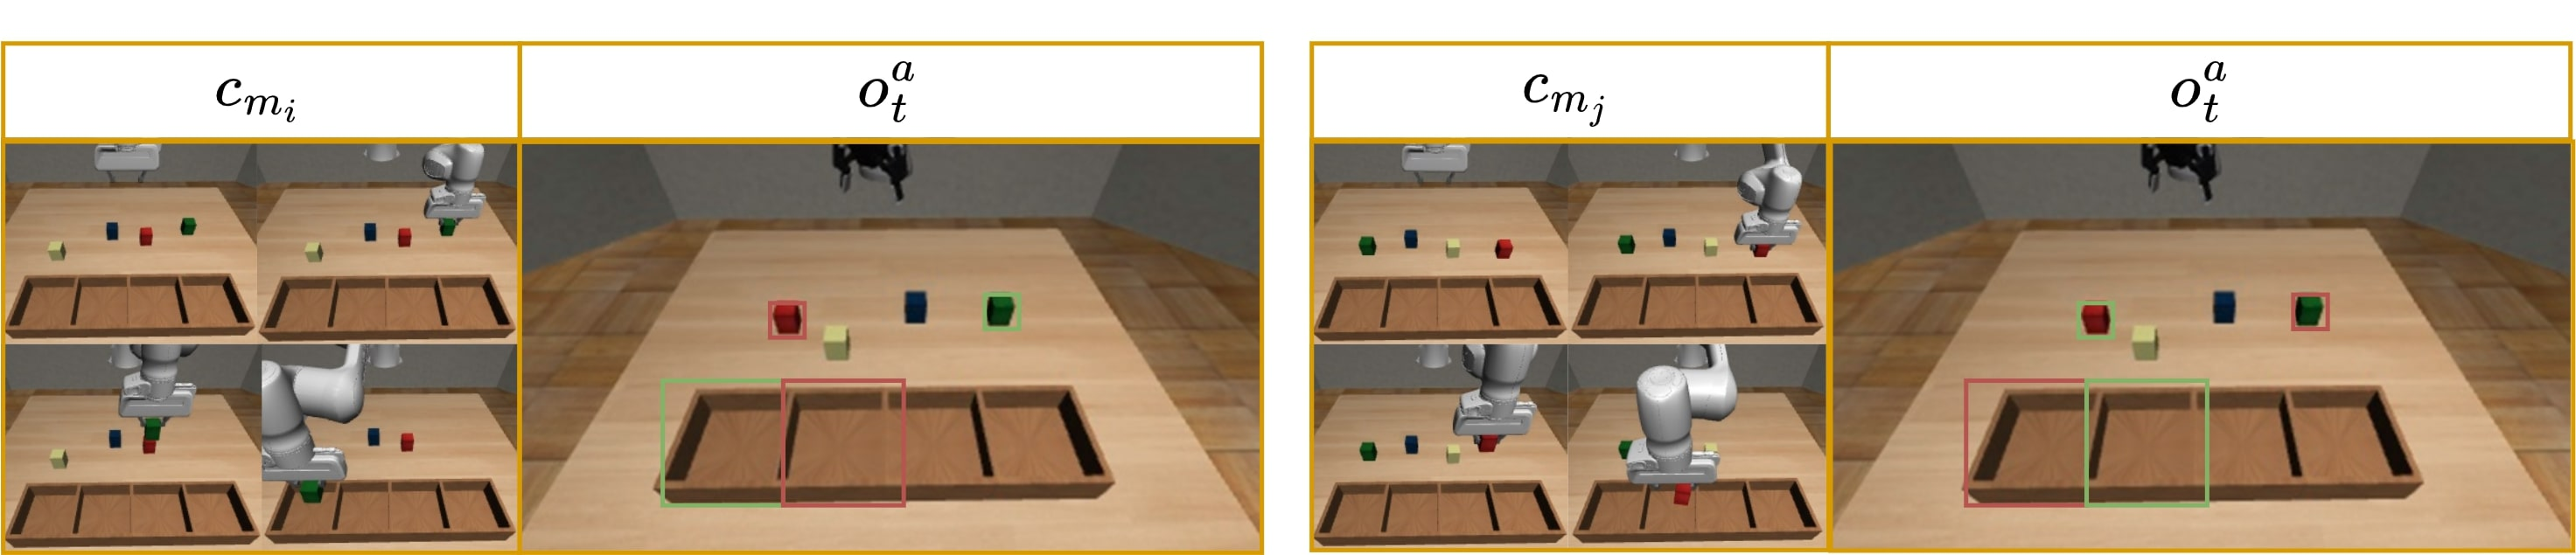
\includegraphics[width=1.0\textwidth]{figures/images/ch2/example_of_bb.jpg}
    \caption{Example of bounding-boxes assignment, where green boxes refer to target object and placing location while red boxed refers to no-target and no-target-place. (Left) The demonstrator manipulates the green box, placing it into the first bin. (Right) The demonstrator manipulates the red box, placing it into the second bin. Note, how for a given agent environment state, the semantic attribute between objects changes.}
    \label{fig:example_of_bb}
\end{figure}
